\documentclass{article}

\usepackage[english]{babel}
\usepackage[utf8]{inputenc}
\usepackage{amsmath}
\usepackage{amsthm}
\usepackage{amssymb}
\usepackage{mathtools}
\usepackage{amsfonts}
\usepackage{graphicx}
\usepackage{wrapfig}
\usepackage{bbm}
\usepackage{dsfont}

% set up margin
\usepackage
[
  a4paper,
  left=3cm,
  right=3cm,
  top=3cm,
  bottom=3cm,
]
{geometry}

% set up header
\usepackage{fancyhdr}
\pagestyle{fancy}
\fancyhf{}
\lhead{6.438 Algorithms for Inference}
\chead{Problem Set 3}
\rhead{Hongzi Mao}
\cfoot{\thepage}
\rfoot{\footnotesize{\emph{Collaborated with: Hongzhou Ye, Zhiwei Ding}}}

% footer line
\renewcommand{\footrulewidth}{0.4pt}

% sans serif italic
\newcommand{\s}[1]{\textsf{\textit{#1}}}

% bold face sans serif
\newcommand{\bs}[1]{\textsf{\textbf{#1}}}

% set symbol
\usepackage[mathscr]{euscript}

% empty set
\let\emptyset\varnothing

% qed
\newcommand{\qeds}{\hfill\qedsymbol}

% math bold face
\newcommand{\bm}{\mathbf}

% independence symbol
\makeatletter
\newcommand*{\indep}{%
  \mathbin{%
    \mathpalette{\@indep}{}%
  }%
}
\newcommand*{\nindep}{%
  \mathbin{%                   % The final symbol is a binary math operator
    \mathpalette{\@indep}{\not}% \mathpalette helps for the adaptation
                               % of the symbol to the different math styles.
  }%
}
\newcommand*{\@indep}[2]{%
  \sbox0{$#1\perp\m@th$}%        box 0 contains \perp symbol
  \sbox2{$#1=$}%                 box 2 for the height of =
  \sbox4{$#1\vcenter{}$}%        box 4 for the height of the math axis
  \rlap{\copy0}%                 first \perp
  \dimen@=\dimexpr\ht2-\ht4-.2pt\relax
  \kern\dimen@
  {#2}
  \kern\dimen@
  \copy0 %                       second \perp
} 
\makeatother

%%%%%%%%%%%%%%%%%%%%%%%%%%%%%%%%%%%%%%%%%%%%%%%%%%%%%%%%%%%%%%%%%%%%%%%%
%%%%%%%%%%%%%%%%%%%%%%%%% Begin document here %%%%%%%%%%%%%%%%%%%%%%%%%%
%%%%%%%%%%%%%%%%%%%%%%%%%%%%%%%%%%%%%%%%%%%%%%%%%%%%%%%%%%%%%%%%%%%%%%%%
\begin{document}
 
\section*{Problem 3.1}
%
(a) When marginalizing Gaussian variables, the variance term carries from the joint covariance.
As a result, for variables $\s{x}_i, \s{x}_j$ with no connection on covariance graph, the covariance
matrix has $0$ on all entries off the diagonal. Therefore, all unconditional independencies are
%$\begin{bmatrix}
%    \Lambda_{ii} & 0 \\
%    0 & \Lambda_{ij}
%\end{bmatrix}$. 
\begin{equation*}
	\s{x}_1 \indep \s{x}_3, \; \s{x}_1 \indep \s{x}_4,\; \s{x}_2 \indep \s{x}_4.
\end{equation*}
The corresponding covariance matrix is
$\bm{\Lambda} = \begin{bmatrix}
    \Lambda_{11} & \Lambda_{12} & 0 & 0 \\
    \Lambda_{21} & \Lambda_{22} & \Lambda_{23} & 0 \\
    0 & \Lambda_{32} & \Lambda_{33} & \Lambda_{34} \\
    0 & 0 & \Lambda_{43} & \Lambda_{44}
\end{bmatrix}$. Thus, in general, the information matrix $\bm{J} = \bm{\Lambda}^{-1}$ has
non-zero values for all entries. In order words, the undirected graph is fully connected.
Hence, there is no conditional independencies.
\\
\\


\noindent
(b) To abuse the notation, we use $\bm{\Lambda}_{i,j,\cdots,k}$ to indicate the covariance matrix of variables $\s{x}_i, \s{x}_j, \cdots, \s{x}_k$. Thus, the covariance matrix for $\s{x}_1, \s{x}_2, \s{x}_3, \s{x}_4$ is
$\bm{\Lambda}_{1, 2, 3, 4} = \begin{bmatrix}
    \Lambda_{11} & 0 & \Lambda_{13} & 0 \\
    0 & \Lambda_{22} & 0 & \Lambda_{24} \\
    \Lambda_{31} & 0 & \Lambda_{33} & 0 \\
    0 & \Lambda_{42} & 0 & \Lambda_{44}
\end{bmatrix}$, and the corresponding covariance graph is shown in Figure~\ref{f:1b}.
\begin{figure}[h]
  \centering
  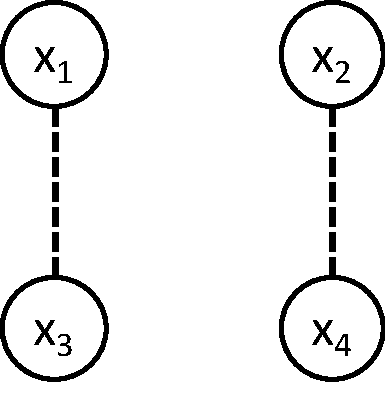
\includegraphics[width=0.2\columnwidth]{1b.pdf}
    \vspace{-0.1cm}
  \caption{Covariance graph with the fewest possible edges for $p_{\s{x}_1, \s{x}_2, \s{x}_3, \s{x}_4}$.}
  \label{f:1b}
\end{figure}
\\
\\

\noindent
(c) Notice that $\bm{\Lambda}_{5,6} =
\begin{bmatrix}
    \Lambda_{55} & 0 \\
    0 & \Lambda_{66}
\end{bmatrix}$
%
and
%
$\bm{\Lambda}_{(5,6), (1,2,3,4)} = \bm{\Lambda}_{(1,2,3,4), (5,6)}^T =
\begin{bmatrix}
    \Lambda_{51} & \Lambda_{52} & 0 & 0 \\
    0 & 0 & \Lambda_{63} & \Lambda_{64}
\end{bmatrix}$. Thus, 
$\bm{\Lambda}_{(1,2,3,4), (5,6)}\bm{\Lambda}_{5,6}^{-1} \bm{\Lambda}_{(5,6), (1,2,3,4)}
\simeq
\begin{bmatrix}
    * & * & 0 & 0 \\
    * & * & 0 & 0 \\
    0 & 0 & * & * \\
    0 & 0 & * & *
\end{bmatrix}$,
where ``$*$'' denotes non-zero values. Hence, the covariance matrix for
$\s{x}_1, \s{x}_2, \s{x}_3, \s{x}_4 | \s{x}_5, \s{x}_6$ \,is\;
$\bm{\Lambda}_{(1,2,3,4)} + \bm{\Lambda}_{(1,2,3,4), (5,6)}\bm{\Lambda}_{5,6}^{-1} \bm{\Lambda}_{(5,6), (1,2,3,4)}
\simeq
\begin{bmatrix}
    * & * & * & 0 \\
    * & * & 0 & * \\
    * & 0 & * & * \\
    0 & * & * & *
\end{bmatrix}$.
The corresponding covariance graph is shown in Figure~\ref{f:1c}.
\begin{figure}[h]
  \centering
  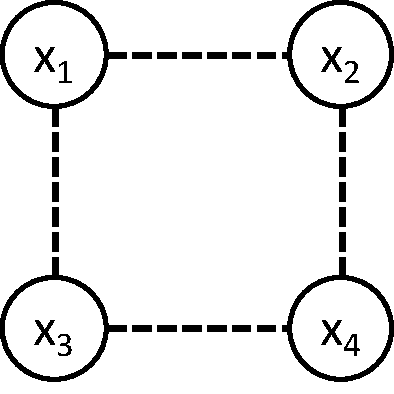
\includegraphics[width=0.2\columnwidth]{1c.pdf}
    \vspace{-0.1cm}
  \caption{Covariance graph with the fewest possible edges for
  $p_{\s{x}_1, \s{x}_2, \s{x}_3, \s{x}_4|\s{x}_5, \s{x}_6}$.}
  \label{f:1c}
\end{figure}
\pagebreak

%%%%%%%%%%%%%%%%%%%%%%%%%%%%%%%%%%%%%%%%%%%%%%%%%%%%%%%%%%%%%%%%%%%%%%%%%%%%%%%%%%%%%%%%
\section*{Problem 3.2}
(a) Suppose $\bs{x}_1$ and $\bs{z}$ are independent and their information matrix is
$\bm{J}' =
\begin{bmatrix}
    \bm{J}_{11}' & 0 \\
    0 & \bm{J}_{22}'
\end{bmatrix}$, potential vector is $[\bm{h}_1'\,^T, \bm{h}_2'\,^T]\,^T$. Now,
\begin{align*}
p_{\bs{x}_1, \bs{x}_2}(\bm{x}_1, \bm{x}_2) &= 
p_{\bs{x}_1, \bs{z}}(\bm{x}_1, \bm{x}_2 + \bm{A}\bm{x}_1) \\
&\propto
\exp\left\{ -\frac{1}{2}
\begin{bmatrix}
    \bm{x}_1^T & \bm{x}_2^T + \bm{x}_1^T \bm{A}^T
\end{bmatrix}
\begin{bmatrix}
    \bm{J}_{11}' & 0 \\
    0 & \bm{J}_{22}'
\end{bmatrix}
\begin{bmatrix}
    \bm{x}_1 \\
    \bm{x}_2 + \bm{A}\bm{x}_1
\end{bmatrix} + 
\begin{bmatrix}
    \bm{h}_1'^T & \bm{h}_2'^T
\end{bmatrix}
\begin{bmatrix}
    \bm{x}_1 \\
    \bm{x}_2 + \bm{A}\bm{x}_1
\end{bmatrix}
\right\}\\
&\propto \exp \bigg[
-\frac{1}{2}\left(
\bm{x}_1^T\bm{J}_{11}'\bm{x}_1 +
\bm{x}_2^T\bm{J}_{22}'\bm{x}_2 +
\bm{x}_2^T\bm{J}_{22}'\bm{A}\bm{x}_1 +
\bm{x}_1^T\bm{A}^T\bm{J}_{22}'\bm{x}_2 +
\bm{x}_1^T\bm{A}^T\bm{J}_{22}'\bm{A}\bm{x}_1
\right) \\
&\;\;\;\;\;+ \bm{h}_1'^T \bm{x}_1
+ \bm{h}_2'^T \bm{x}_2
+ \bm{h}_2'^T \bm{A}\bm{x}_1 \bigg].
\end{align*}
%
Meanwhile, 
%
\begin{align*}
p_{\bs{x}_1, \bs{x}_2}(\bm{x}_1, \bm{x}_2) &\propto \exp\left\{ -\frac{1}{2}
\begin{bmatrix}
    \bm{x}_1^T & \bm{x}_2^T 
\end{bmatrix}
\begin{bmatrix}
    \bm{J}_{11} & \bm{J}_{12} \\
    \bm{J}_{21} & \bm{J}_{22}
\end{bmatrix}
\begin{bmatrix}
    \bm{x}_1 \\
    \bm{x}_2
\end{bmatrix} + 
\begin{bmatrix}
    \bm{h}_1^T & \bm{h}_2^T
\end{bmatrix}
\begin{bmatrix}
    \bm{x}_1 \\
    \bm{x}_2
\end{bmatrix}
\right\}\\
&\propto\exp\left[
-\frac{1}{2}\left(
\bm{x}_1^T\bm{J}_{11}\bm{x}_1 +
\bm{x}_1^T\bm{J}_{12}\bm{x}_2 +
\bm{x}_2^T\bm{J}_{21}\bm{x}_1 +
\bm{x}_2^ T\bm{J}_{22}'\bm{x}_2
\right) + 
\bm{h}_1^T \bm{x}_1 +
\bm{h}_2^T \bm{x}_2
\right].
\end{align*}
%
Thus, by term matching,
%
\begin{align*}
	\bm{J}_{22}' &= \bm{J}_{22}, \\
	\bm{J}_{22}'\bm{A} &= \bm{J}_{21} \implies \bm{A} = \bm{J}_{22}^{-1}\bm{J}_{21}, \\
	\bm{J}_{11}' + \bm{A}^T\bm{J}_{22}'\bm{A} &= \bm{J}_{11},\\ % \implies \bm{J}_{11}' = \bm{J}_{11} - \bm{A}^T\bm{J}_{22}\bm{A}, \\
	\bm{h}_2' &= \bm{h}_2,\\
	\bm{h}_1' &= \bm{h}_1 - \bm{A}^T\bm{h}_2.
\end{align*}
Since $\bs{x}_1$ and $\bs{z}$ are independent, $\bs{x}_1 \sim \mathscr{N}^{-1}(\bm{J}_{11}', \bm{h}_{1}')$.
By plugging in $\bm{A} = \bm{J}_{22}^{-1}\bm{J}_{21}$ from above, and knowing
$\bm{J}_{11}$ and $\bm{J}_{22}$ being symmetric, and $\bm{J}_{12}^T =\bm{J}_{21}$, we have
\begin{align*}
	\bm{J}_{11}' &= \bm{J}_{11} - \bm{A}^T\bm{J}_{22}\bm{A} = \bm{J}_{11} - \bm{J}_{12}\bm{J}_{22}^{-1}\bm{J}_{21},\\
	\bm{h}_1' &= \bm{h}_1 - \bm{J}_{12}\bm{J}_{22}^{-1}\bm{h}_2.
\end{align*}

\noindent
(b) Let
\begin{align*}
\begin{bmatrix}
    \bm{J}_{11} & \bm{J}_{12} \\
    \bm{J}_{21} & \bm{J}_{22}
\end{bmatrix}
\begin{bmatrix}
    \bm{m}_{1}\\
    \bm{m}_{2}
\end{bmatrix} = 
\begin{bmatrix}
    \bm{h}_{1}\\
    \bm{h}_{2}
\end{bmatrix},
\end{align*}
which brings
\begin{align*}
	&\bm{J}_{11}\bm{m}_1 + \bm{J}_{12}\bm{m}_2 = \bm{h}_1\\
	&\bm{J}_{21}\bm{m}_1 + \bm{J}_{22}\bm{m}_2 = \bm{h}_2.
\end{align*}
%
From the second equation above, we have
\begin{align*}
	\bm{m}_2 = \bm{J}_{22}^{-1}(\bm{h}_2 - \bm{J}_{21}\bm{m}_1).
\end{align*}
%
Plugging in the first equation,
\begin{align*}
	\bm{J}_{11}\bm{m}_1 + \bm{J}_{12}\bm{J}_{22}^{-1}(\bm{h}_2 - \bm{J}_{21}\bm{m}_1) = \bm{h}_1.
\end{align*}
Rearranging,
\begin{align*}
	\left(\bm{J}_{11} + \bm{J}_{12}\bm{J}_{22}^{-1}\bm{J}_{21}\right)\bm{m}_1 = \bm{h}_1 - \bm{J}_{12}\bm{J}_{22}^{-1}\bm{h}_2.
\end{align*}
\\

\noindent
(c)(i) Notice that
\begin{align*}
p_{\bs{x}_1, \bs{x}_2, \bs{x}_3}(\bm{x}_1, \bm{x}_2, \bm{x}_3) &\propto	
\exp\left\{-\frac{1}{2}\left(
\begin{bmatrix}
    \bm{x}_1^T & \bm{x}_2^T & \bm{x}_3^T 
\end{bmatrix}
\begin{bmatrix}
    \bm{J}_{11} & \bm{J}_{12} & \bm{J}_{13}\\
    \bm{J}_{21} & \bm{J}_{22} & 0 \\
    \bm{J}_{31} & 0 & \bm{J}_{33}\\
\end{bmatrix}
\begin{bmatrix}
    \bm{x}_1 \\
    \bm{x}_2 \\
    \bm{x}_3
\end{bmatrix}\right) + 
\begin{bmatrix}
    \bm{h}_1^T & \bm{h}_2^T & \bm{h}_3^T
\end{bmatrix}
\begin{bmatrix}
    \bm{x}_1 \\
    \bm{x}_2 \\
    \bm{x}_3
\end{bmatrix}
\right\} \\
&\propto \exp\bigg[-\frac{1}{2}\left(
\bm{x}_1^T\bm{J}_{11}\bm{x}_1 +
\bm{x}_1^T\bm{J}_{12}\bm{x}_2 +
\bm{x}_1^T\bm{J}_{13}\bm{x}_3 +
\bm{x}_2^T\bm{J}_{21}\bm{x}_1 +
\bm{x}_2^T\bm{J}_{22}\bm{x}_2 +
\bm{x}_3^T\bm{J}_{31}\bm{x}_3 +
\bm{x}_3^T\bm{J}_{33}\bm{x}_3
\right)\\
&\;\;\;\; + \bm{h}_1^T\bm{x}_1 + \bm{h}_2^T\bm{x}_2 + \bm{h}_3^T\bm{x}_3 \bigg] \\
&\propto \underbrace{\exp\left[-\frac{1}{2}\left(
\bm{x}_1^T\bm{J}_{11}\bm{x}_1 +
\bm{x}_1^T\bm{J}_{12}\bm{x}_2 +
\bm{x}_2^T\bm{J}_{21}\bm{x}_1 +
\bm{x}_2^T\bm{J}_{22}\bm{x}_2
\right) + \bm{h}_1^T\bm{x}_1 + \bm{h}_2^T\bm{x}_2
\right]}_{h(\bm{x}_1, \bm{x}_2)}\\
&\times \underbrace{\exp\left[-\frac{1}{2}\left(
\bm{x}_1^T\bm{J}_{13}\bm{x}_3 +
\bm{x}_3^T\bm{J}_{31}\bm{x}_3 +
\bm{x}_3^T\bm{J}_{33}\bm{x}_3
\right) + \bm{h}_3^T\bm{x}_3 \right]}_{g(\bm{x}_1, \bm{x}_3)}.
\end{align*}

Hence,
%
$\bs{x}_2 \indep \bs{x}_3 \,|\, \bs{x}_1.$ \qeds
\\

\noindent
(ii) Directly using equation (2), we have
\begin{align*}
	\bm{J}_b &= \bm{J}_{11} -
\begin{bmatrix}
    \bm{J}_{12} & \bm{J}_{13} 
\end{bmatrix}
\begin{bmatrix}
    \bm{J}_{22} & 0 \\
    0 & \bm{J}_{33}
\end{bmatrix}^{-1}
\begin{bmatrix}
    \bm{J}_{21} \\
    \bm{J}_{31}
\end{bmatrix} \\
&= \bm{J}_{11} -
\begin{bmatrix}
    \bm{J}_{12} & \bm{J}_{13} 
\end{bmatrix}
\begin{bmatrix}
    \bm{J}_{22}^{-1} & 0 \\
    0 & \bm{J}_{33}^{-1}
\end{bmatrix}
\begin{bmatrix}
    \bm{J}_{21} \\
    \bm{J}_{31}
\end{bmatrix}\\
&= \bm{J}_{11} - \bm{J}_{12}\bm{J}_{22}^{-1}\bm{J}_{21} - \bm{J}_{13}\bm{J}_{33}^{-1}\bm{J}_{31},
\end{align*}
and
\begin{align*}
	\bm{h}_b &= \bm{h}_1 - 
\begin{bmatrix}
    \bm{J}_{12} & \bm{J}_{13} 
\end{bmatrix}
\begin{bmatrix}
    \bm{J}_{22} & 0 \\
    0 & \bm{J}_{33}
\end{bmatrix}^{-1}
\begin{bmatrix}
    \bm{h}_{2} \\
    \bm{h}_{3}
\end{bmatrix} \\
&= \bm{h}_1 - 
\begin{bmatrix}
    \bm{J}_{12} & \bm{J}_{13} 
\end{bmatrix}
\begin{bmatrix}
    \bm{J}_{22}^{-1} & 0 \\
    0 & \bm{J}_{33}^{-1}
\end{bmatrix}
\begin{bmatrix}
    \bm{h}_{2} \\
    \bm{h}_{3}
\end{bmatrix} \\
&=\bm{J}_{11} - \bm{J}_{12}\bm{J}_{22}^{-1}\bm{h}_{2} - \bm{J}_{13}\bm{J}_{33}^{-1}\bm{h}_{3}.
\end{align*}\qeds
\pagebreak

%%%%%%%%%%%%%%%%%%%%%%%%%%%%%%%%%%%%%%%%%%%%%%%%%%%%%%%%%%%%%%%%%%%%%%%%%%%%%%%%%%%%%%%%
\section*{Problem 3.3}
\end{document}